\chapter{Автоматизированные системы контроля радиационной обстановки}

\section{Необходимость \ac{ascro}}

С каждым годом количество промышленных предприятий в мире стремительно увеличивается. К сожалению, увеличение количества 
промышленных предприятий сопровождается увеличением промышленных выбросов в атмосферу, из-за чего происходит загрязнение 
окружающей среды. Развитие производств, связанных с атомной энергетикой, также связано с проблемой загрязнения 
окружающей среды, особенно в случае радиационных аварий. В связи с этим, одной из главных задач атомной энергетики 
является повышение радиационной безопасности действующих \ac{aes}, а также других \ac{oiae} (\acl{oiae}).

Даже при изолированной от окружающей среды технологии производства на предприятиях атомной энергетики, есть вероятность 
возникновения внештатных ситуаций, приводящих к радиоактивным выбросам и загрязнению окружающей среды. Примерами могут 
служить следующие радиационные аварии, произошедшие в прошлом:

\begin{itemize}
	\item взрыв ёмкостей с радиоактивными отходами на химкомбинате <<Маяк>> (Челябинская область, СССР) 29 сентября 
		1957 г.;
	\item авария на заводе <<Селлафильд>> (Уиндскейл, Великобритания) 10 октября 1957 г.;
	\item авария на \ac{aes} <<Tree Mile Island>> (штат Пенсильвания, США) 28 марта 1979 г.;
	\item авария на Чернобыльской \ac{aes} 26 апреля 1986 г.;
	\item авария на заводе Tokaimura (Токай, Япония) 30 сентября 1999 г.;
	\item авария на \ac{aes} Фукусима-1 (Окума, Япония) 11 марта 2011 г.
\end{itemize}

Примеры выше показывают важность и актуальность задачи радиационного контроля внешней среды вблизи \ac{aes}, 
осуществляемого автоматизированной системой контроля радиационной обстановки. 

\section{Цели и задачи \ac{ascro}}

Основной целью \ac{ascro} является обеспечение руководства \ac{aes} информацией, которая способствует минимизации 
последствий радиационной аварии на \ac{aes} \cite{elokhin}.

Задачами системы являются:

\begin{itemize}
	\item оперативное обнаружение повышенного или аварийного выброса радиоактивных веществ;
	\item прогнозирование распространения радиоактивных выбросов, а также загрязнения окружающей среды;
	\item измерение значений мощности дозы фотонного излучения на прилегающей к \ac{aes} местности;
	\item оценка дозовых нагрузок на персонал и население;
	\item выдача рекомендаций по принятию решений о защите населения.
\end{itemize}

Функционирование системы должно осуществляться в режиме реального времени (on-line), что достигается за счет 
автоматизированного сбора данных при помощи установленных датчиков. Впоследствии, на основе полученных данных 
осуществляется прогностические расчеты с использованием математических моделей распространения радиоактивных примесей в 
атмосфере.

\section{\ac{ascro} на различных этапах развития атомной энергетики}

Развитие автоматизированных систем контроля радиационной обстановки происходило вместе с развитием средств контроля
(таких как детекторы ионизирующих излучений, анализаторы спектра $\alpha$, $\beta$, $\gamma$ излучений), вычислительных 
мощностей \ac{evm}, средств отображения, обработки, хранения и передачи информации, а также с развитием средств 
математического моделирования прогнозирования радиационной обстановки в атмосфере.

Автоматизированные системы контроля радиационной обстановки делятся на три основных поколения \cite{elokhin}.

К первому поколению относятся системы, разрабатываемые до 1960-х годов. Эти системы были построены, в основном, на 
основе автоматических пороговых детекторов, задачей которых являлось сигнализирование при превышении допустимого уровня 
загрязнения окружающей среды. Системы контроля первого поколения ориентировались в основном на осуществление контроля 
за загрязнением внешней среды, вызванным работой \ac{aes} в штатном режиме. Причиной развития такого подхода служил тот 
факт, что радиоактивные выбросы и сбросы \ac{aes} на столько малы за счет систем локализации и подавления активности, 
что они практически не изменяют радиационную обстановку внешней среды.

Системы второго поколения, развитие которых происходило в период с 1960-х до 1980-х годов, содержали в себе еще один 
важный компонент - вычислительный центр со специальным программным обеспечением, позволяющий на основе метеорологических 
данных атмосферы прогнозировать радиационные характеристики во внешней среде. 

Автоматизированные системы контроля радиационной обстановки третьего поколения развиваются по сей день в условиях 
интенсивного совершенствования мощностей вычислительной техники. Из-за развития мощностей становится возможным 
использование более усовершенствованных математических моделей переноса радиоактивных примесей в атмосфере, которые 
позволяют проводить более точное и детальное прогнозирование радиационных характеристик внешней среды.

\section{Состав и принцип работы \ac{ascro}}

Основу \ac{ascro} составляют средства контроля. Входящие в состав системы средства контроля разделяют на 
метеорологические и радиационные \cite{elokhin}.

Метеорологические средства контроля включат в себя совокупность датчиков метеопараметров, по показаниям которых 
определяют такие параметры, как направление ветра, продольная и поперечная составляющие скорости ветра, температура и 
влажность воздуха. На основе этих параметров также определяют состояние устойчивости атмосферы, которое оказывает 
большое влияние на распространение радиоактивных примесей в атмосфере. Кроме того, перечисленные параметры входят в 
уравнение адвекции-диффузии, которое используется при разработке модели \ac{ascro} в текущей работе. Именно поэтому 
измерение указанных метеопараметров является необходимым для выполнения корректных расчетов, позволяющих прогнозировать 
радиационные характеристики внешней среды. Как правило, метеорологические параметры атмосферы измеряют на метеоплощадках, 
на которых установлены метеорологические мачты, предназначенные для измерения скорости ветра и температуры.

Радиационный контроль во внешней среде осуществляется при помощи датчиков фотонного излучения (БДМГ-08Р3, БДМГ-08Р4, 
БДМГ-08Р5), располагающихся на промплощадке в пределах 1-1,5 км от \ac{aes}. Датчики фотонного излучения имеют кабельную 
связь по специально выделенным линиям, а также по коммутируемым телефонным линиям. В случае расположения датчиков на 
расстоянии, превышающем 1,5 км, используются телефонная связь и радиосвязь на ультракоротких волнах по выделенному 
частотному диапазону.

Поскольку ведущим средством измерения \ac{ascro} являются гамма-датчики, то при увеличении их количества на промплощадке 
вблизи \ac{aes} повышается надежность и достоверность информации о радиационной обстановке. В то же время, каждый 
установленный датчик для нормальной работы требует основные и дополнительные линии связи электропитания, автономного 
питания, а также другое оборудование, стоимость которого является ключевым среди затрат на систему. В связи с этим 
ставится задача оптимизации количества датчиков фотонного излучения с экономической точки зрения и с точки зрения 
качества информации о радиационной обстановке вблизи \ac{aes}.

Не менее важным параметром при решении уравнения переноса радиоактивных примесей в атмосфере является мощность выброса 
радиоактивных газоаэрозольных примесей, поступающих в атмосферу через вентиляционные трубы \ac{aes}. Величину мощности 
выброса в атмосферу через вентиляционные трубы [Бк/c] определяют согласно формуле \ref{eq_P_v} \cite{elokhin}:

\begin{equation}
    \label{eq_P_v}
    P = G \times A_{v0} \sum_{i=1}^{N} p_i
\end{equation}

где:
\begin{description}
    \item $G$ --- секундный расход газоаэрозольных выбросов [м$^3$/с];
    \item $p_i$ --- вес i-ого нуклида в смеси газоаэрозольных выбросов;
    \item $A_{v0}$ --- полная объемная активность радионуклидов газоаэрозольных выбросов.
\end{description}

Для измерения мощности газоаэрозольных выбросов на \ac{aes} используются специальные датчики. Примером такого вида 
датчиков может служить датчик, представляющий собой спаренные проточную и непроточную ионизационные камеры одинаковых 
размеров и с одинаковым объемом рабочего пространства (рисунок \ref{fig_P_detector}). Проточная и непроточная камеры 
используется для измерения скорости воздушного потока по разности ионизационных токов в точке расположения детекторов. 
Кроме того, непроточная камера применяется для оценки мощности дозы фотонного излучения. Датчики мощности радиоактивных 
выбросов устанавливают в устье вентиляционных труб \ac{aes}.

\begin{figure}[ht!]
	\centering
	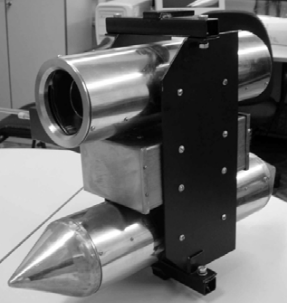
\includegraphics[width=8cm]{P_detector}
	\captionsetup{justification=centering}
    \caption{Датчик мощности радиоактивных выбросов \ac{aes} \cite{elokhin}.}
    \label{fig_P_detector}
\end{figure}

Исходные данные, полученные из вышеописанных средств контроля, передаются в расчетную математическую модель,  
представляющую собой набор специальных математических программ, установленных в вычислительных центрах и предназначенных 
для прогностических расчетов переноса радиоактивных примесей в атмосфере, а также оценки уровней радиоактивного 
загрязнения подстилающей поверхности, дозовых нагрузок на персонал и население в условиях радиационных аварий.

На основе выходных характеристик расчетной модели принимается решение о необходимости эвакуации населения из 
загрязненного района вблизи \ac{aes}. В случае необходимости проведения эвакуации решается задача выбора оптимального 
пути следования автотранспортных средств при эвакуации населения, а также количество автотранспортных средств, водителей 
и число рейсов, необходимое для проведения эвакуации.

Структурная схема \ac{ascro} представлена на рисунке \ref{fig_ascro_scheme}.

\begin{figure}[ht!]
	\centering
	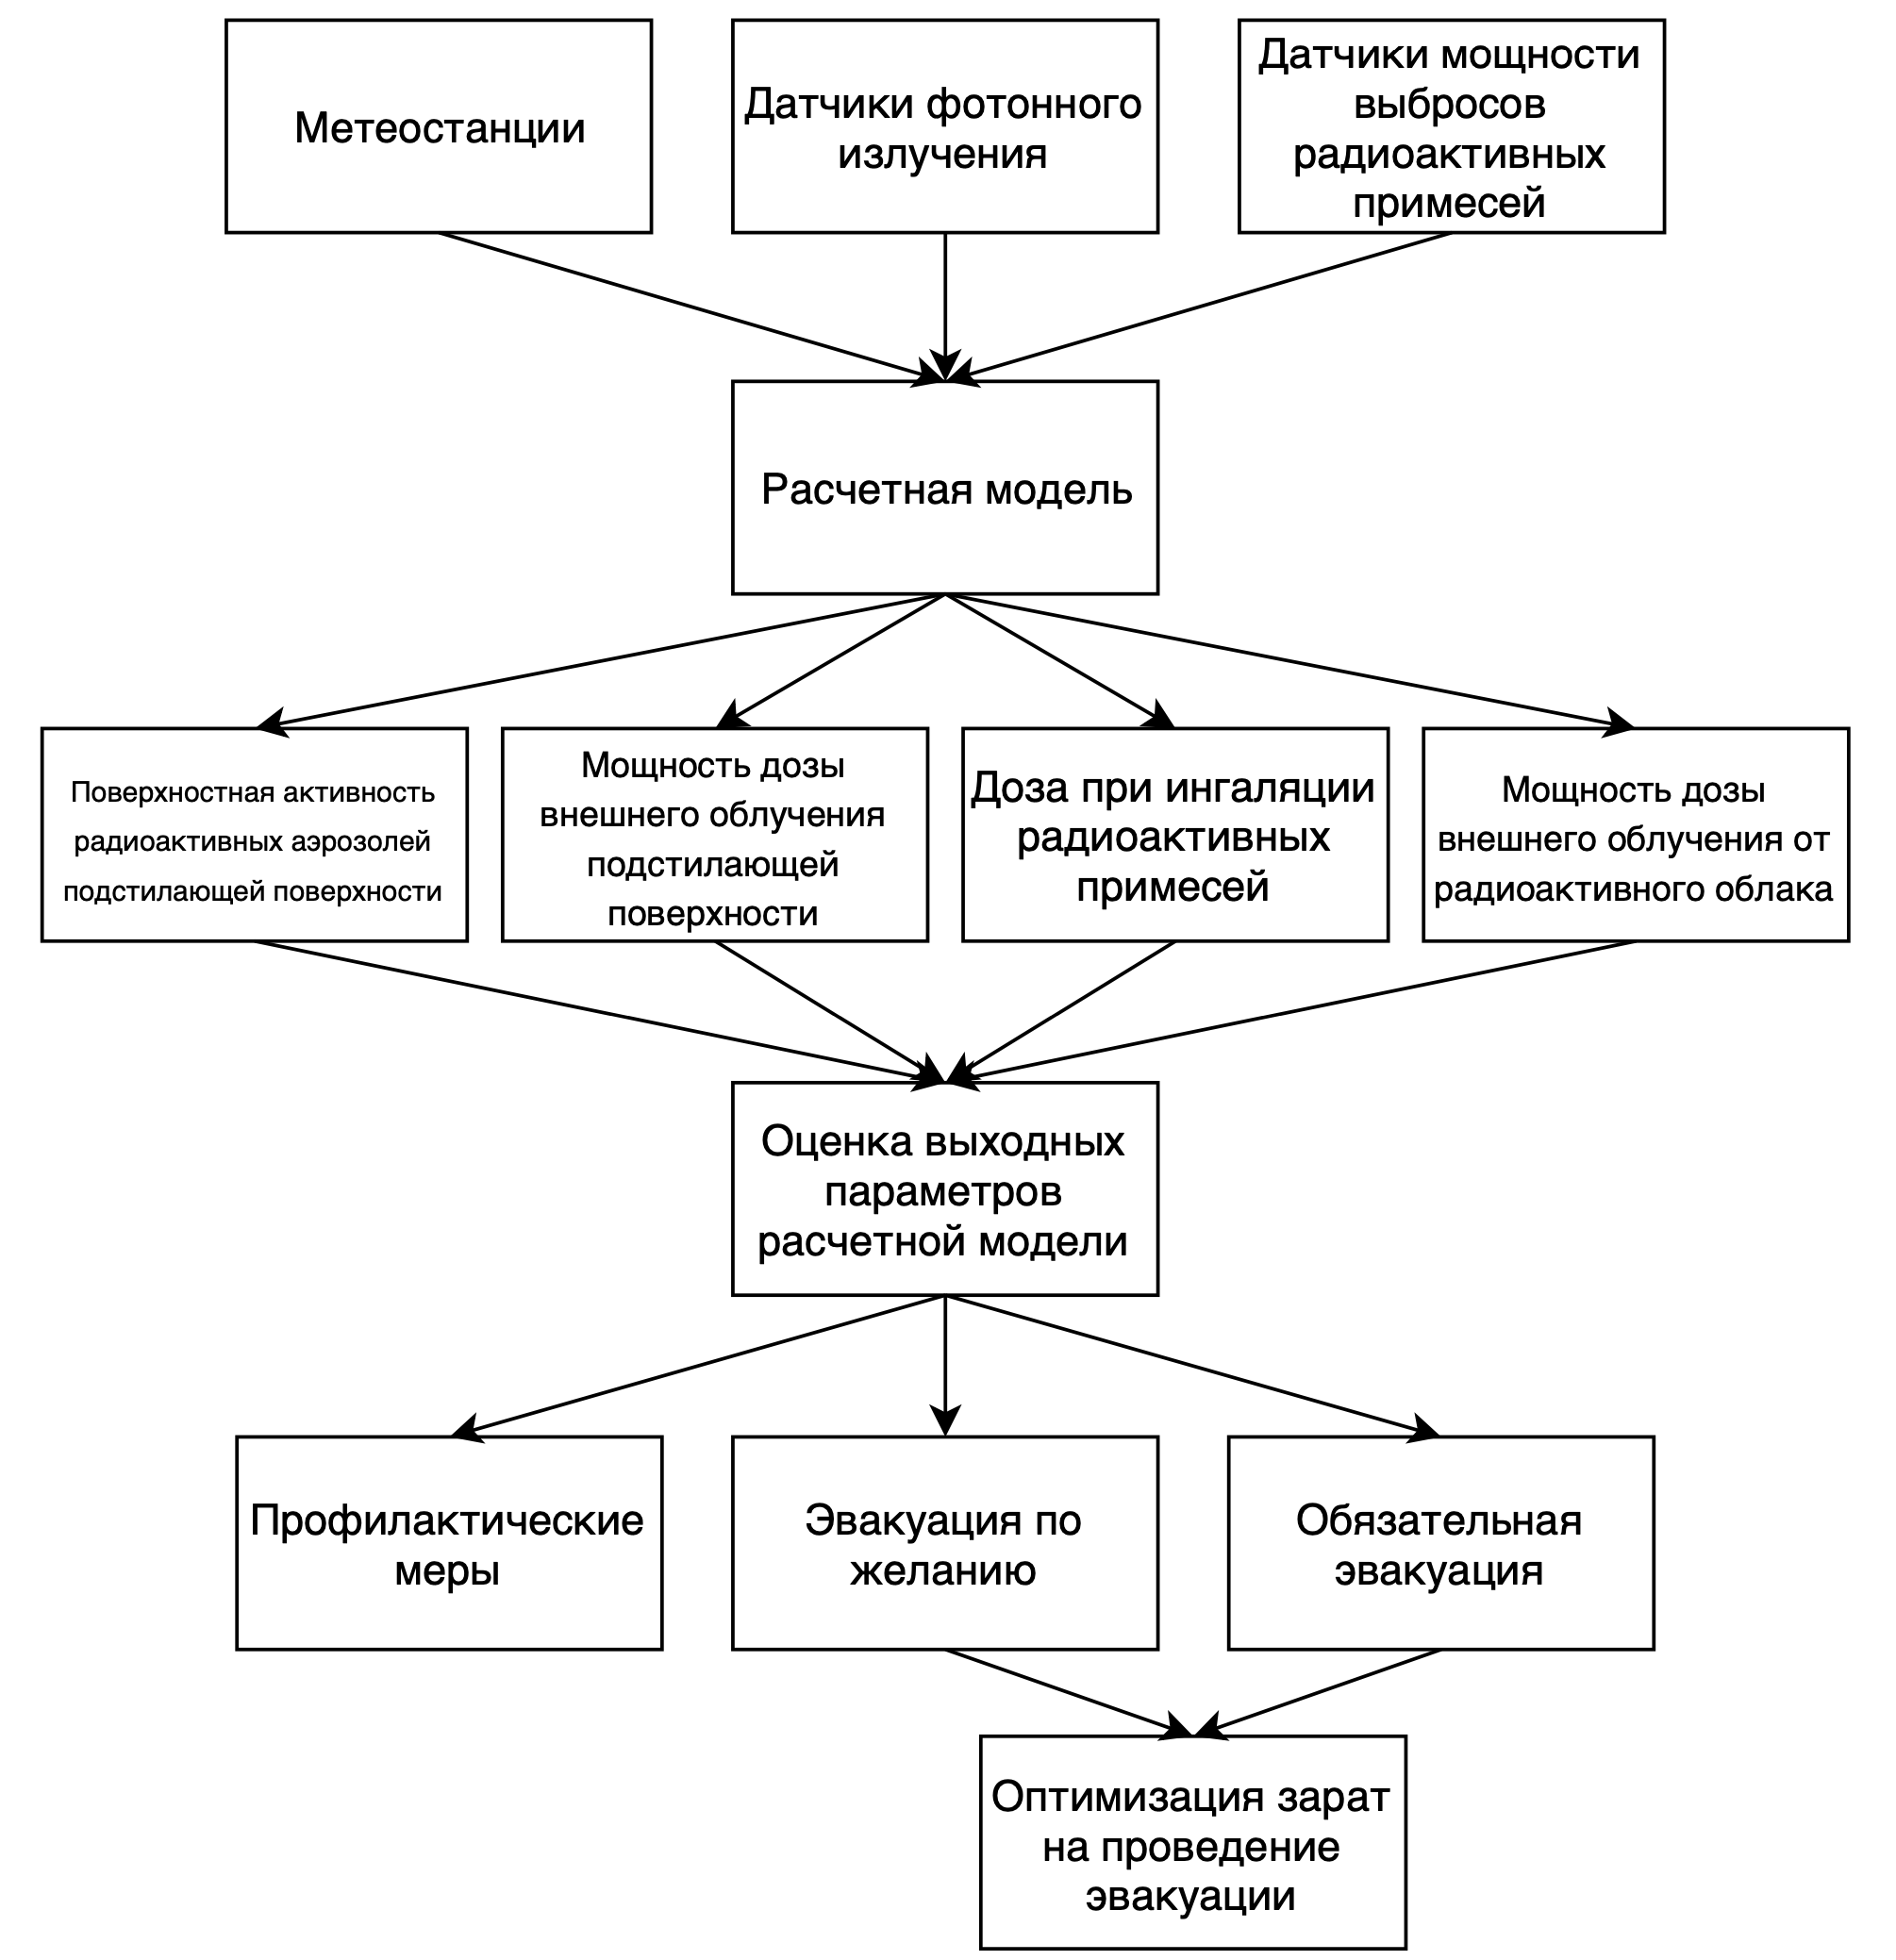
\includegraphics[width=17cm]{ascro_scheme}
	\captionsetup{justification=centering}
    \caption{Структурная схема \ac{ascro} \cite{elokhin}.}
    \label{fig_ascro_scheme}
\end{figure}

\section{Заключение обзора \ac{ascro}}

В данной главе было приведено краткое введение в автоматизированные системы контроля радиационной обстановки. В начале 
было показано, почему разработка \ac{ascro} является важной и актуальной задачей для атомной энергетики при 
строительстве атомных электростанций. Далее были описаны основные цели и задачи, которые решаются посредством 
автоматизированных систем контроля радиационной обстановки. Было представлено совершенствование \ac{ascro} на различных 
этапах развития атомной энергетики, а также состав \ac{ascro} и принцип её работы.